\section{Rešerše a analýza existujícíh OpenSource aplikací}

Při hledání existujících aplikací jsem hledal za pomocí umělé inteligence. Použil jsem tento dotaz: \textit{"Is there any open source app that gathers open data about IAQ or IEQ"}. Jako odpověď jsem dostal: 

\textit{"Yes, here are a few open-source apps/tools for IAQ (Indoor Air Quality) or IEQ (Indoor Environmental Quality):}
\begin{enumerate}
	\item{\textit{AirCasting
		Gathers IAQ data via sensors like the AirBeam.
		Open-source  and \newline community-driven.
		GitHub: AirCasting.}}
	
	\item{\textit{OpenSenseMap
		Platform for environmental data, including air quality.
		Supports DIY sensor integrations.
		Website: opensensemap.org.}}
	
	\item{\textit{Luftdaten.info (Sensor Community)
		Collects and visualizes IAQ data from DIY sensors.
		Open-source hardware and software.
		GitHub: Luftdaten.}}
	
	\item{\textit{Sensor.Community
		Continuation of Luftdaten for broader environmental monitoring.
		Community-powered data sharing.
		Website: sensor.community.}}
\end{enumerate}
\textit{These tools combine IAQ data collection, visualization, and community involvement}"\newline \parencite{openaiChatGPT2024}.


Při výběru aplikace, která by měla podobné vlastnosti, které jsou zmíněny v cílech byla vybrány 2 aplikace.

\subsection{Aplikace 1 - sensor.community}

 První je na portále \textit{sensor.community}, který byl dříve znám jako Luftdaten. Jedná se o projekt ze Štuttgartu v Německu. Aplikace umožňuje lidem se registrovat a připojit své nízkonákladové senzory k této síti. Aplikace podporuje širokou škálu senzorů a vývojových desek. Na webovém portále si lze zobrazit mapu světa (viz obrázek \ref{obr01:sens-com-map}) , kde lze sledovat hladiny různých veličin na základě umístění (viz obrázek \ref{obr02:sens-com-veliciny-a-data}). Co však nelze, je zobrazení grafů vývoje. A to ani v portálu uživatele, kde uživatel může spravovat svá zařízení. Data jsou zde spíše obecná, to dává v kontextu otevřených dat smysl, ale jistá personalizace pro uživatele by mohla existovat.

\begin{figure}[h!]
	\centering
	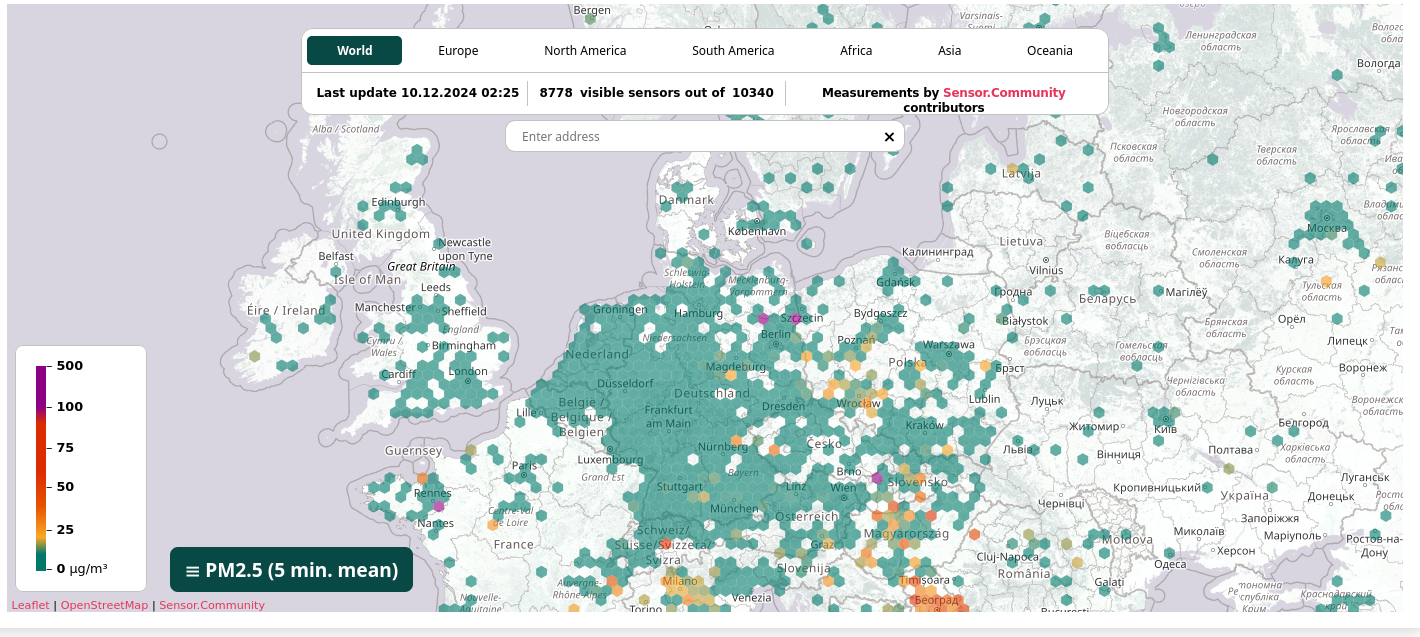
\includegraphics[width=.70\textwidth]{img/sensor-community-map.png}

	\caption{Mapa senzorů na webu sensor.community}
	\label{obr01:sens-com-map}
\end{figure}

\begin{figure}[h!]
	\centering
	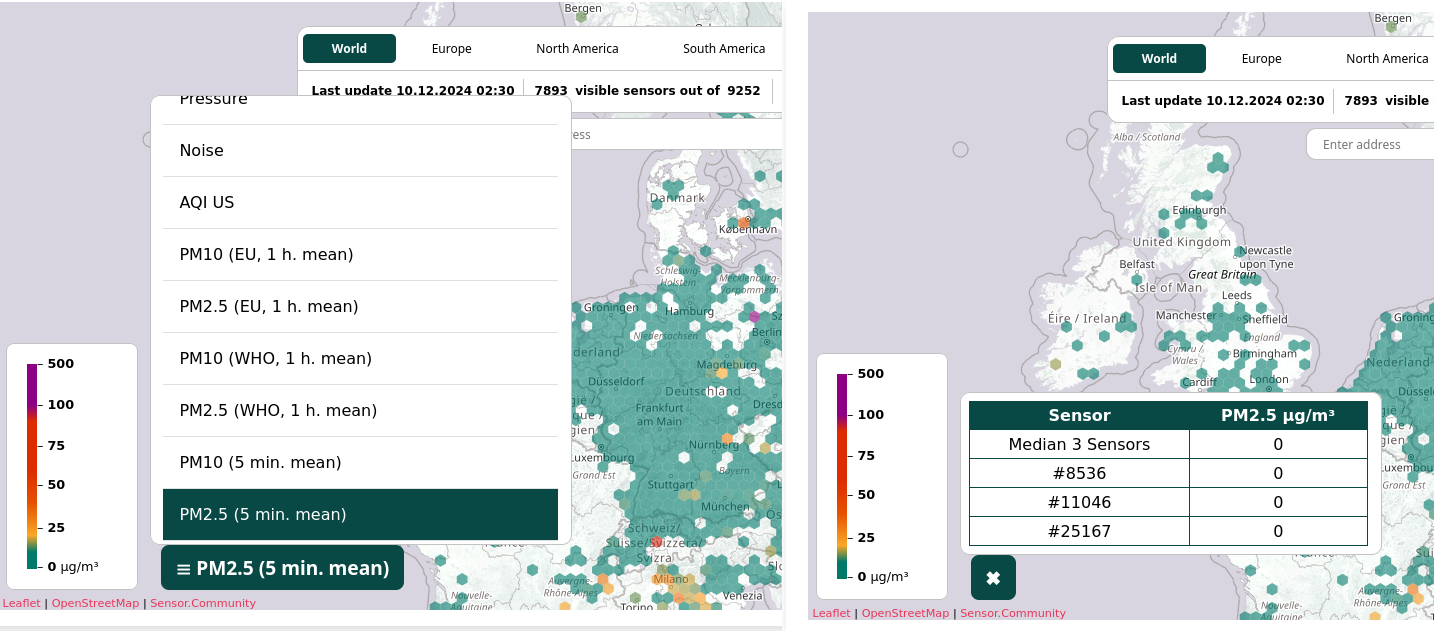
\includegraphics[width=.70\textwidth]{img/sensor-community-veliciny-a-data.png}
	\caption{Ukázka měřených veličin a vizualizace dat na webu sensor.community}
	\label{obr02:sens-com-veliciny-a-data}
\end{figure}

\subsection{Aplikace 2 - opensensemap.org}

Druhou aplikací je portál opensensemap.org. Tato aplikace nabízí velmi podobné funkce jako ta předchozí. Má však nějaké funkce navíc. Již se dá zobrazit grafy pro jednotlivé veličiny senzoru. Stále zde není možnost nahlížen na své senzory přímo z dashboardu. Pouze z globální mapy. I přes pěkné vizuální zpracování aplikace a více funkcemi oproti předchozí aplikaci, jsou zde jisté neduhy. Aplikace postrádá standardizaci pro data vznikají tak často duplicity. Filtrování podlé \textit{fenoménu}, jak aplikace různé veličiny nazývá, je prakticky nemožné něco efektivně filtrovat. Jen pro teplotu se zde nachází desítky \textit{fenoménů}. Tento problém přisuzuji přílišné volnosti poskytnuté uživateli v případě poskytování dat.


\subsection{Shrnutí}
Obě aplikace jsou shodou okolností německého původu, jsou tedy primárně v německém jazyce a překlad do angličtiny či češtiny pokulhává.

